\usepackage{tikz}
\usetikzlibrary{calc}
\usepackage{tikzpagenodes}
\usepackage{fancyhdr}

\renewcommand{\headrulewidth}{0pt}
\renewcommand{\footrulewidth}{0pt}

\aliaspagestyle{plain}{empty}
\aliaspagestyle{chapter}{toc}

\newcommand{\makeheader}[1]{%
  \begin{tikzpicture}[remember picture,overlay]
  \draw node [inner sep=0,outer sep=0,below right] 
        at (current page.north west){\includegraphics[width=\paperwidth]{#1}};
  \end{tikzpicture}
}

\newcommand{\makefooter}[1]{%
  \begin{tikzpicture}[remember picture,overlay]
  \draw node [inner sep=0,outer sep=0,above right] 
        at (current page.south west){\includegraphics[width=\paperwidth]{#1}};
  \end{tikzpicture}
}

\newcommand{\tlflower}[1][flower]{%
\begin{tikzpicture}[remember picture,overlay]
\draw node [inner sep=0,outer sep=0,below right] 
at (current page.north west){\includegraphics[width=0.3\paperwidth]{images/#1-tl-corner}};
\end{tikzpicture}}

\newcommand{\trflower}[1][flower]{%
\begin{tikzpicture}[remember picture,overlay]
\draw node [inner sep=0,outer sep=0,below left] 
at (current page.north east){\includegraphics[width=0.3\paperwidth]{images/#1-tr-corner}};
\end{tikzpicture}}

\newcommand{\brflower}[1][flower]{%
\begin{tikzpicture}[remember picture,overlay]
\draw node [inner sep=0,outer sep=0,above left] 
at (current page.south east){\includegraphics[width=0.3\paperwidth,angle=-90]{images/#1-tr-corner}};
\end{tikzpicture}}

\newcommand{\blflower}[1][flower]{%
\begin{tikzpicture}[remember picture,overlay]
\draw node [inner sep=0,outer sep=0,above right] 
at (current page.south west){\includegraphics[width=0.3\paperwidth,angle=90]{images/#1-tl-corner}};
\end{tikzpicture}}

\newcommand{\makecenterflourish}[2][0]{%
  \begin{tikzpicture}[remember picture,overlay]
  \draw node [inner sep=0,outer sep=0,above] 
    at ([xshift=0.5\paperwidth,yshift=#1\paperheight]current page.south west){\includegraphics[width=0.5\paperwidth]{#2}};
\end{tikzpicture}}

\fancypagestyle{title}{%
  \fancyhf{}%
  % \begin{tikzpicture}[remember picture,overlay]
  % \draw node [inner sep=0,outer sep=0,below right] 
  %       at (current page.north west){
\includegraphics[width=\paperwidth,angle=180]{images/flower-footer}};
  % % \draw node [inner sep=0,outer sep=0,above right] 
  % %       at (current page.south west){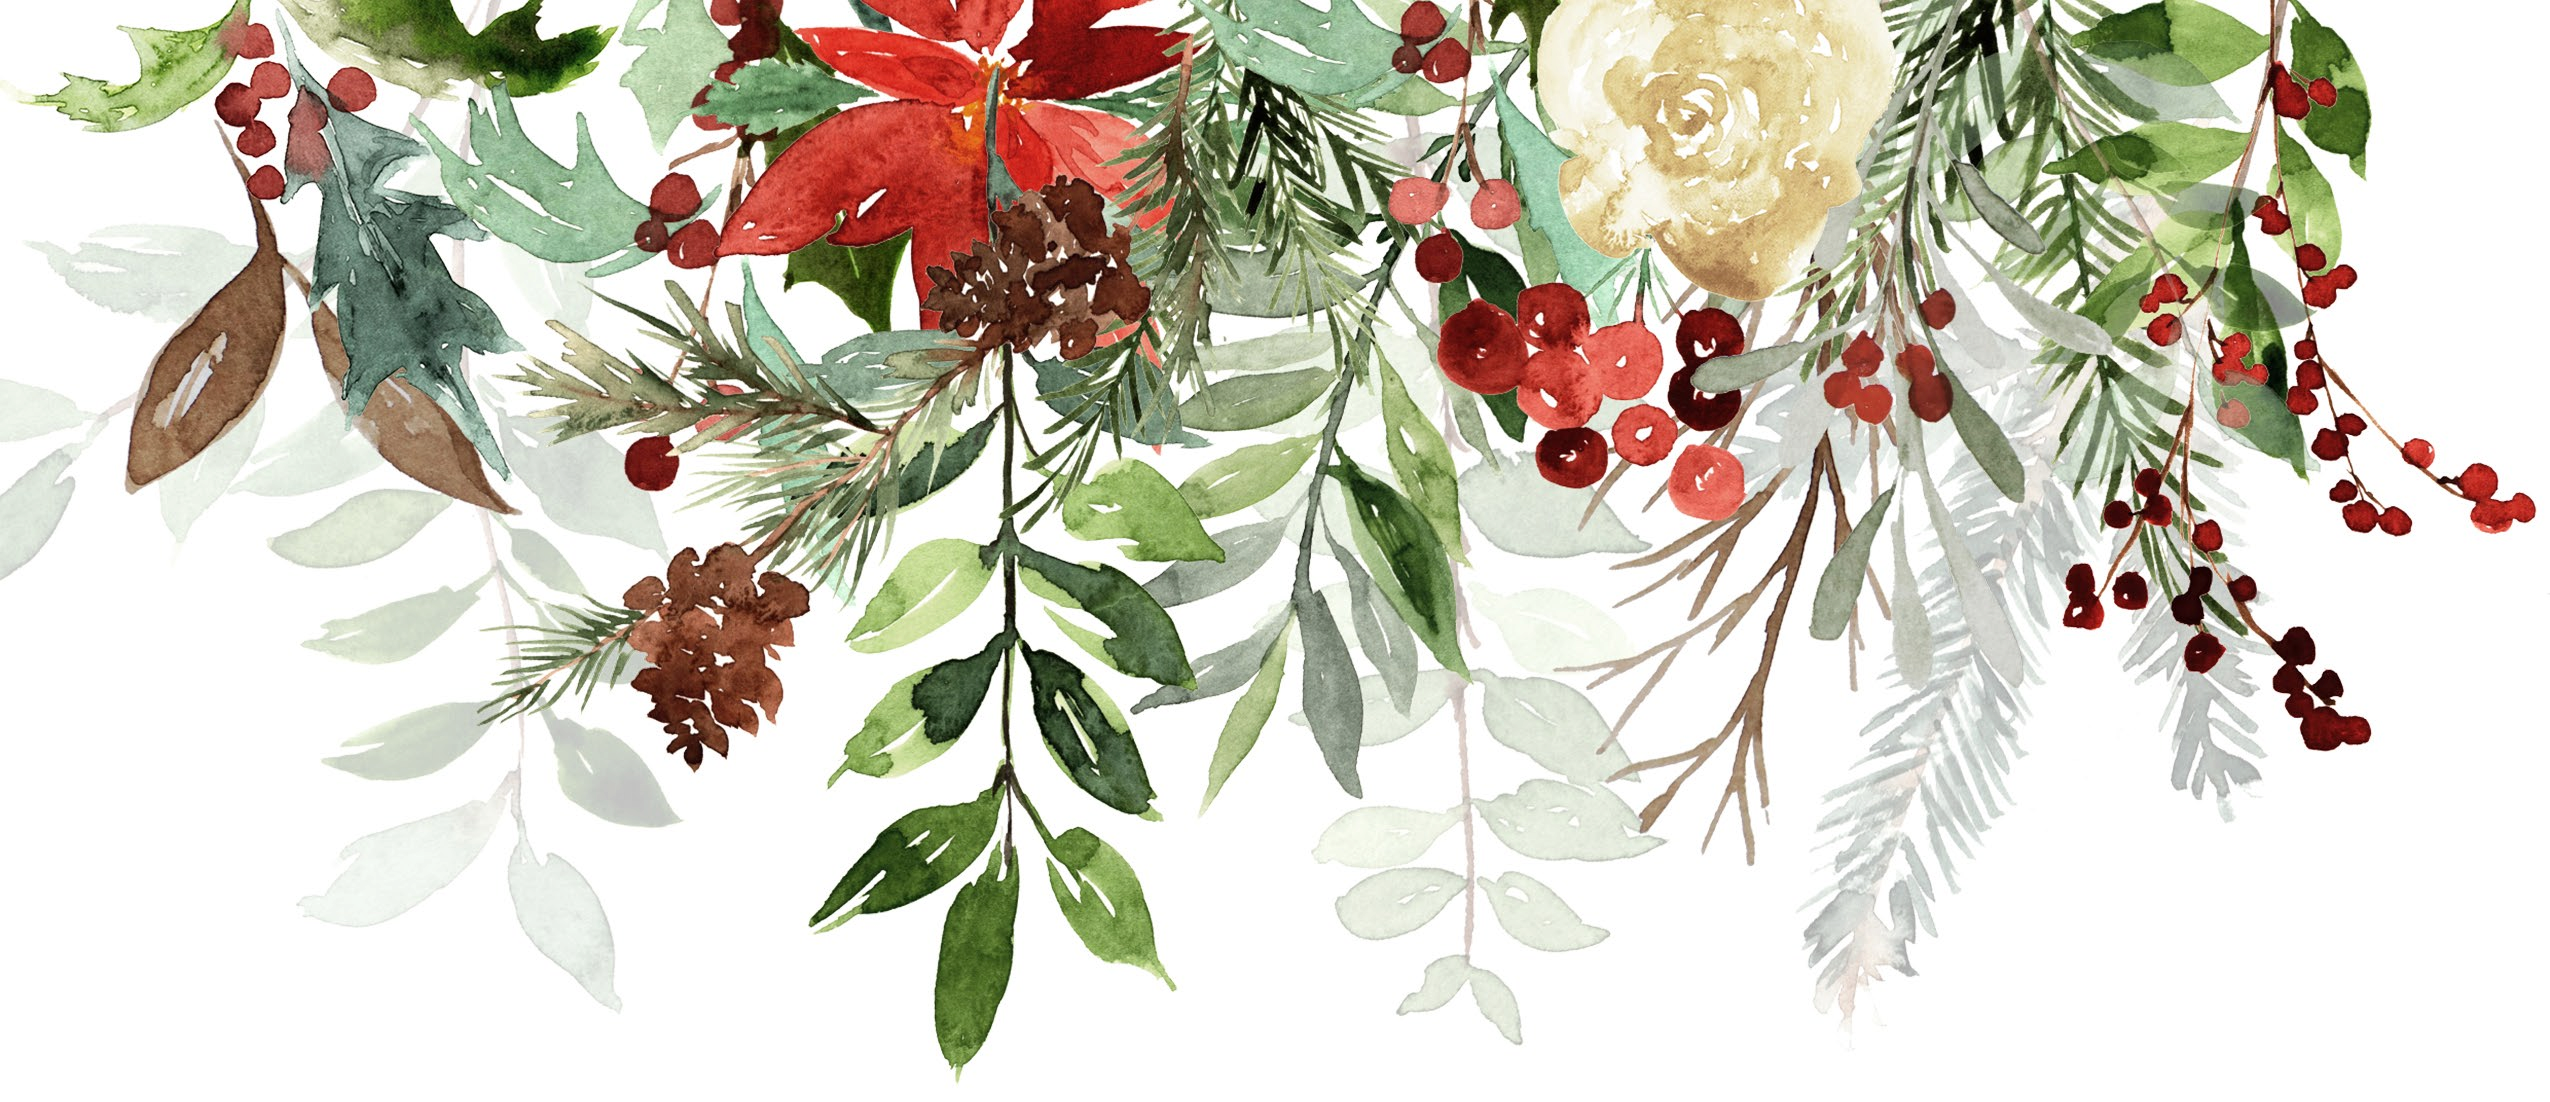
\includegraphics[width=\paperwidth,angle=180]{images/flower-header-2}};
  % \end{tikzpicture}
  \makecenterflourish[0.6]{images/flower-wreath}
  \makefooter{images/flower-footer}
}

\fancypagestyle{toc}{%
  \fancyhf{}%
  \tlflower{}
  \brflower{}
}

\fancypagestyle{flower-headfoot-1}{%
  \fancyhf{}%
  \makeheader{images/flower-header-1}
  \makefooter{images/flower-footer}
  \fancyfoot[R]{\thepage}
}

\fancypagestyle{flower-header-1}{%
  \fancyhf{}%
  \makeheader{images/flower-header-1}
  \fancyfoot[R]{\thepage}
}

\fancypagestyle{flower-lamp-header}{%
  \fancyhf{}%
  \makeheader{images/flower-lamp-header}
  \fancyfoot[R]{\thepage}
}

\fancypagestyle{foliage-header}{%
  \fancyhf{}%
  \makeheader{images/foliage-header}
  \fancyfoot[R]{\thepage}
}

\fancypagestyle{cabin-lamp-header}{%
  \fancyhf{}%
  \makeheader{images/cabin-lamp-header}
  \fancyfoot[R]{\thepage}
}

\fancypagestyle{flower-header-2}{%
  \fancyhf{}%
  \makeheader{images/flower-header-2}
  \fancyfoot[R]{\thepage}
}

\newcommand{\deerfooter}{%
\begin{tikzpicture}[remember picture,overlay]
\draw node [inner sep=0,outer sep=0,above right] 
at ([xshift=-2.5cm]current page.south west){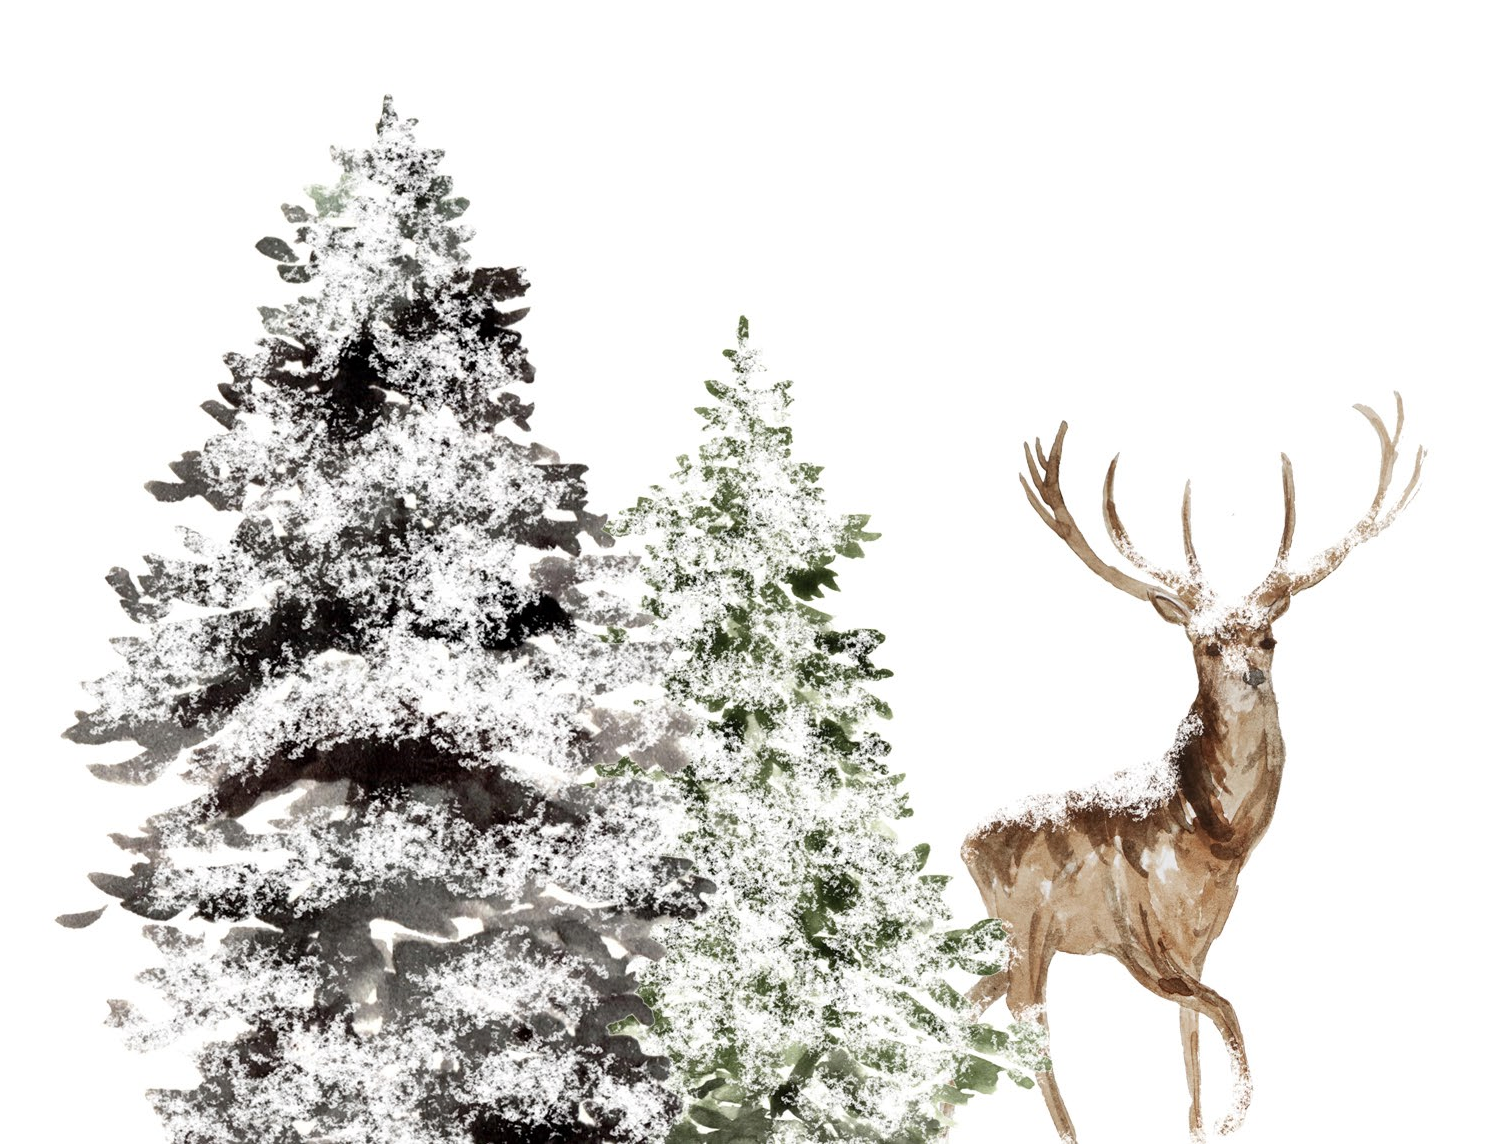
\includegraphics[width=0.7\paperwidth]{images/deer-2}};
\end{tikzpicture}}

